\documentclass[11pt]{article}
\usepackage[a4paper,margin=1in]{geometry}
\usepackage{booktabs}
\usepackage{float}
\usepackage{graphicx}
\usepackage{amsmath}
\usepackage{amssymb}
\usepackage{siunitx}

\graphicspath{{../results/project}}

\title{Laboratory 02 Report: Dataset Analysis}
\author{Machine Learning and Pattern Recognition}
\date{}

\begin{document}
\maketitle

\section{Project Section: Fingerprint Spoofing Dataset}

The project dataset contains 6000 samples, 6 features, and binary labels: 0 for fake fingerprints and 1 for genuine fingerprints.

\section{Analysis of Features 1 and 2}

\subsection*{Empirical Results}

To evaluate the discriminative power of the first two features, we analyze their class-conditional means, variances, 1D histograms, and 2D scatter plots. 

\textbf{Distributions and Overlap:} 
Based on the histograms (\texttt{feature\_1\_histogram.png} and \texttt{feature\_2\_histogram.png}), the distributions for both the "Genuine" (label 1) and "Fake" (label 0) classes are strictly unimodal, exhibiting a single, distinct peak. However, the classes exhibit a massive, nearly total overlap. As seen in the scatter plot (\texttt{features\_1\_2\_scatter.jpg}), both distributions are perfectly centered at the origin $(0,0)$, creating a dense intersecting cluster.

\textbf{Statistical Metrics:}
The computed statistics perfectly reflect this visual overlap:
\begin{itemize}
    \item \textbf{Means:} The means are virtually identical and centered near zero. For Feature 1, the Fake mean is $0.0029$ and Genuine is $0.0005$. For Feature 2, the Fake mean is $0.0187$ and Genuine is $-0.0085$.
    \item \textbf{Variances:} While the means are identical, the variances are heavily inverted between the axes. For Feature 1, the Genuine class has a massive variance ($1.4302$) compared to Fake ($0.5696$). Conversely, for Feature 2, the Fake class has the dominant variance ($1.4209$) compared to Genuine ($0.5783$).
\end{itemize}

\begin{figure}[H]
    \centering
    \begin{minipage}{0.48\textwidth}
        \centering
        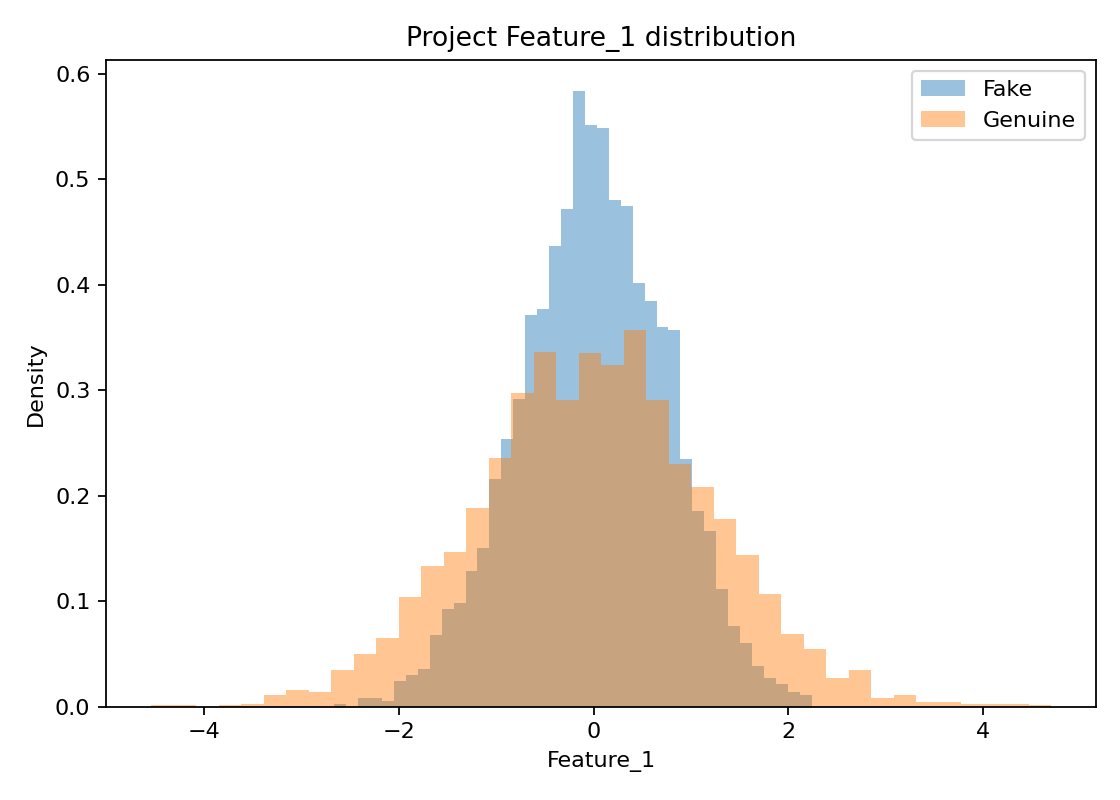
\includegraphics[width=\linewidth]{histograms/feature_1_histogram.png}
        \caption{Histogram of Feature 1.}
    \end{minipage}\hfill
    \begin{minipage}{0.48\textwidth}
        \centering
        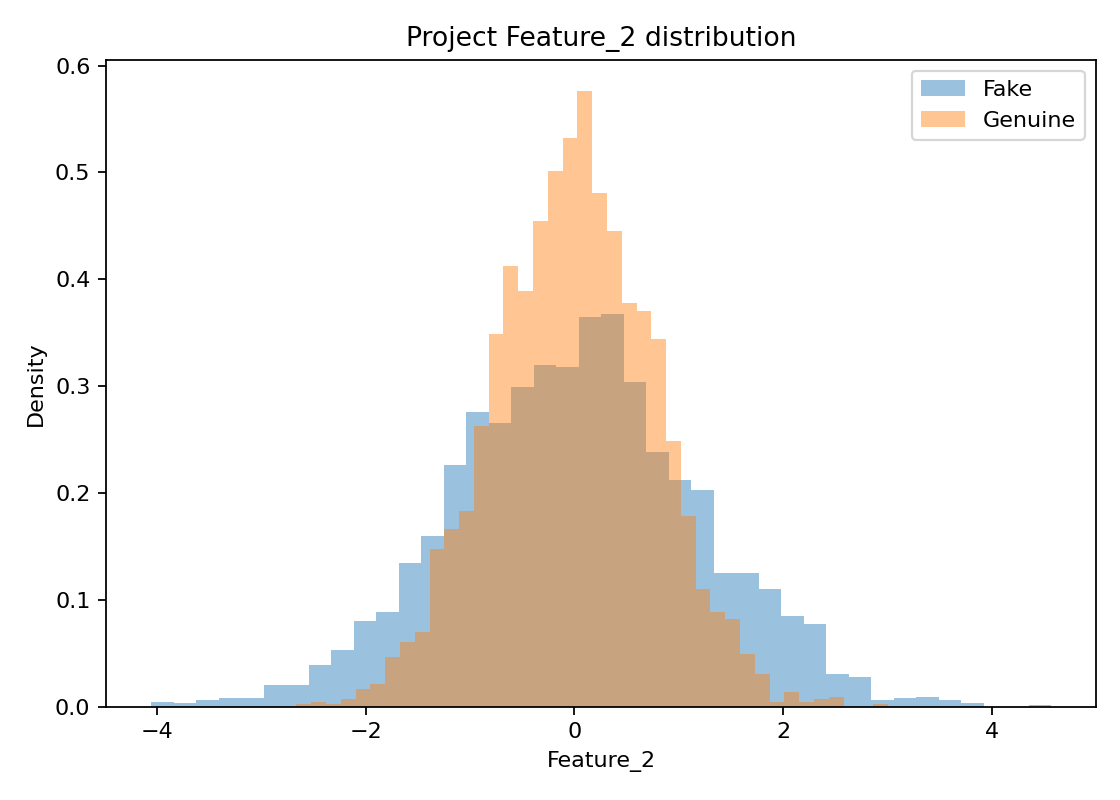
\includegraphics[width=\linewidth]{histograms/feature_2_histogram.png}
        \caption{Histogram of Feature 2.}
    \end{minipage}
\end{figure}

\begin{figure}[H]
    \centering
    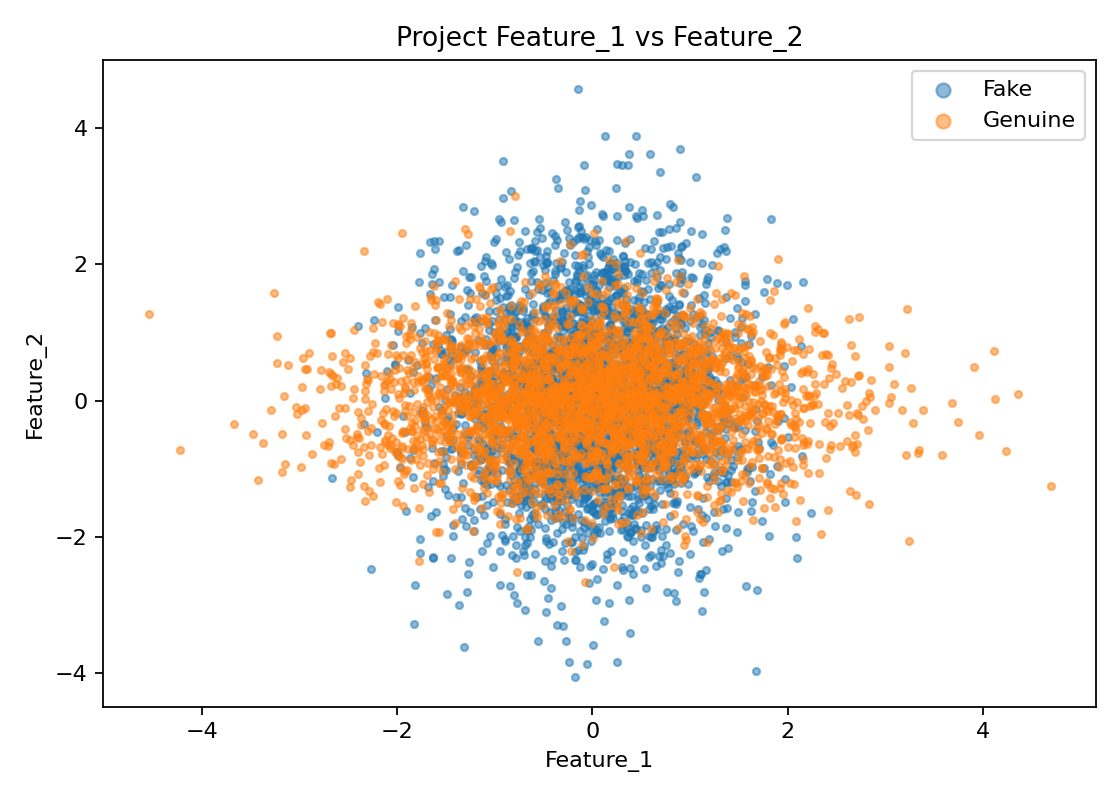
\includegraphics[width=0.6\textwidth]{scatters/features_1_2_scatter.png}
    \caption{Scatter plot of Feature 1 vs Feature 2, illustrating the inverted variance "cross" topology.}
    \label{fig:scatter_1_2}
\end{figure}

\subsection*{Theoretical Analysis}

The statistical inversion of the variances combined with identical means yields a highly specific geometric topology. Because the centers of mass for both classes sit exactly on top of each other at $(0,0)$, there is no spatial shift between them. Instead, the classes differentiate themselves purely by their spread.

The Fake class spreads vertically along the Feature 2 axis, while the Genuine class spreads horizontally along the Feature 1 axis. In a 2D space, this creates a distinct "cross" or "plus-sign" intersection (clearly visible in Figure \ref{fig:scatter_1_2}). 

\subsection*{Motivation and Future Insights}

This specific feature geometry provides critical insight that directly predicts the performance of our classifiers in subsequent laboratories (Lab 6 and Lab 10):

\begin{enumerate}
    \item \textbf{Failure of Linear Models:} Because the centroids are identical, a globally linear decision boundary (like standard Logistic Regression) cannot effectively separate these classes. A straight line drawn through the origin will inevitably misclassify half of the cross.
    \item \textbf{Catastrophic Failure of Tied MVG:} This topology perfectly explains why the Tied Covariance MVG performed so poorly throughout the project. The Tied MVG forces both classes to share a single, averaged covariance matrix. By averaging the horizontal Genuine spread and the vertical Fake spread, the Tied MVG assumes both classes are identical, symmetric circles. It completely destroys the only discriminative geometric information available in these features.
    \item \textbf{Success of Quadratic/Non-Linear Models:} To separate a cross-shaped distribution, a classifier must be able to draw an ellipse or a closed geometric boundary. This theoretically justifies why models capable of generating quadratic boundaries (like the Standard MVG) or highly localized non-linear boundaries (like the RBF Kernel SVM used in our final fusion) vastly outperformed the linear baselines.
\end{enumerate}
\newpage

\section{Analysis of Features 3 and 4}

\subsection*{Empirical Results}

To further evaluate the discriminative landscape of the dataset, we analyze the statistical metrics and spatial distribution of Features 3 and 4.

\textbf{Distributions and Overlap:}
Based on the histograms (\texttt{feature\_3\_histogram.png} and \texttt{feature\_4\_histogram.png}), the distributions for both the Genuine and Fake classes are strictly unimodal, each exhibiting a single, well-defined peak. Observing the scatter plot (\texttt{features\_3\_4\_scatter.jpg}), we see that the classes occupy distinct, opposite quadrants. While there is a margin of overlap in the center $(0,0)$ region, the two distributions are clearly separated along a diagonal axis.

\textbf{Statistical Metrics:}
The computed statistics perfectly reflect this diagonal separation and structural similarity:
\begin{itemize}
    \item \textbf{Means:} The means are highly distinct and perfectly inverted between the classes. For the Fake class, the centroid is located in the top-left quadrant at Feature 3 = $-0.6809$ and Feature 4 = $0.6708$. For the Genuine class, the centroid is mirrored into the bottom-right quadrant at Feature 3 = $0.6652$ and Feature 4 = $-0.6642$.
    \item \textbf{Variances:} In stark contrast to Features 1 and 2, the variances here are remarkably symmetric. The variance for the Fake class is $0.5500$ (Feature 3) and $0.5360$ (Feature 4), while the Genuine class exhibits nearly identical variances of $0.5489$ (Feature 3) and $0.5533$ (Feature 4).
\end{itemize}

\begin{figure}[H]
    \centering
    \begin{minipage}{0.48\textwidth}
        \centering
        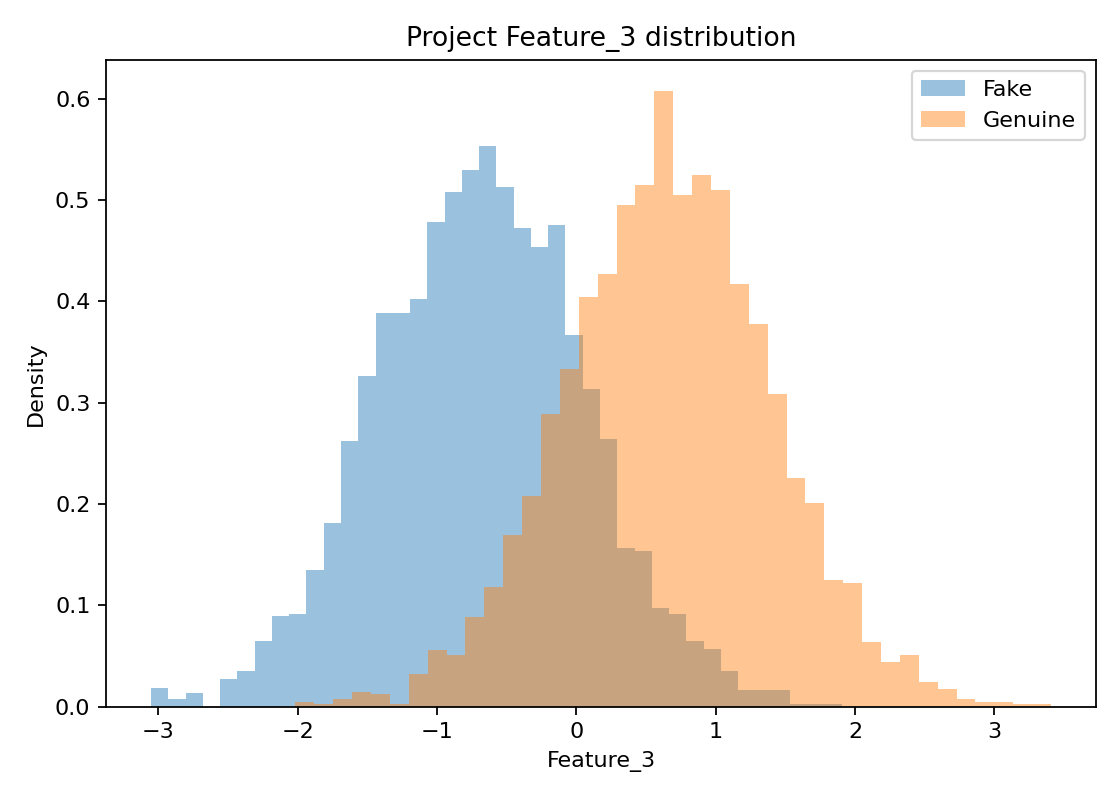
\includegraphics[width=\linewidth]{histograms/feature_3_histogram.png}
        \caption{Histogram of Feature 3.}
    \end{minipage}\hfill
    \begin{minipage}{0.48\textwidth}
        \centering
        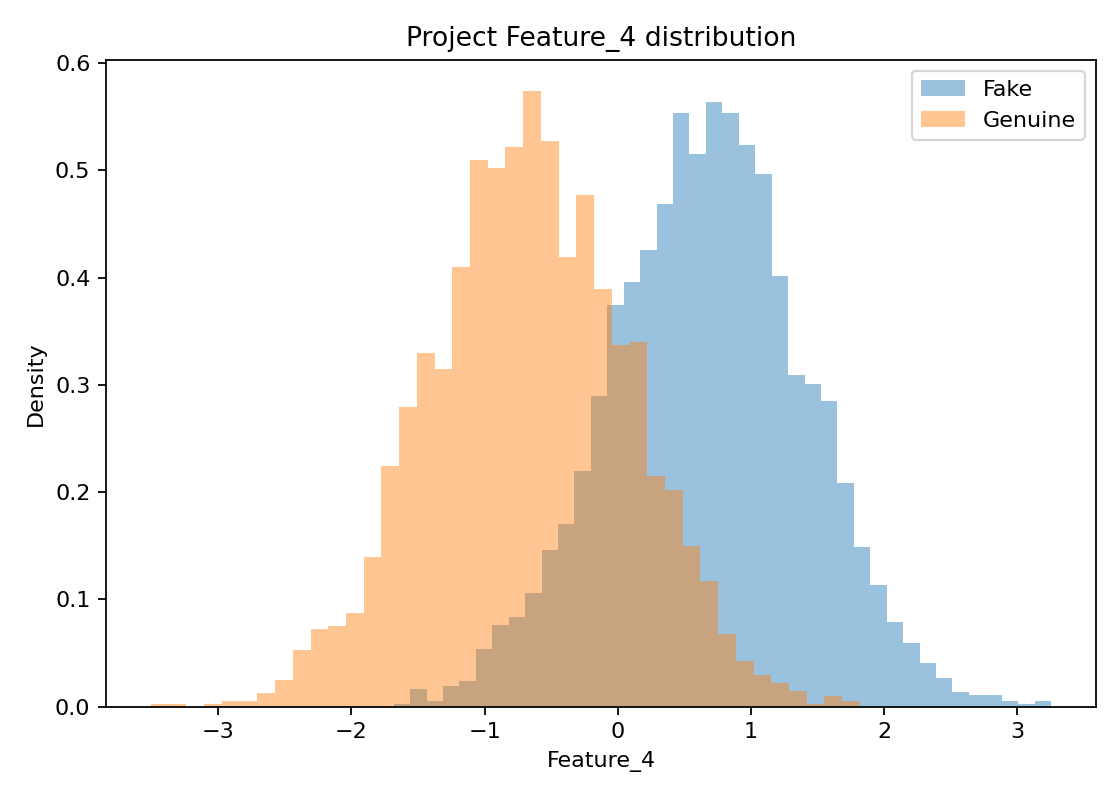
\includegraphics[width=\linewidth]{histograms/feature_4_histogram.png}
        \caption{Histogram of Feature 4.}
    \end{minipage}
\end{figure}

\begin{figure}[H]
    \centering
    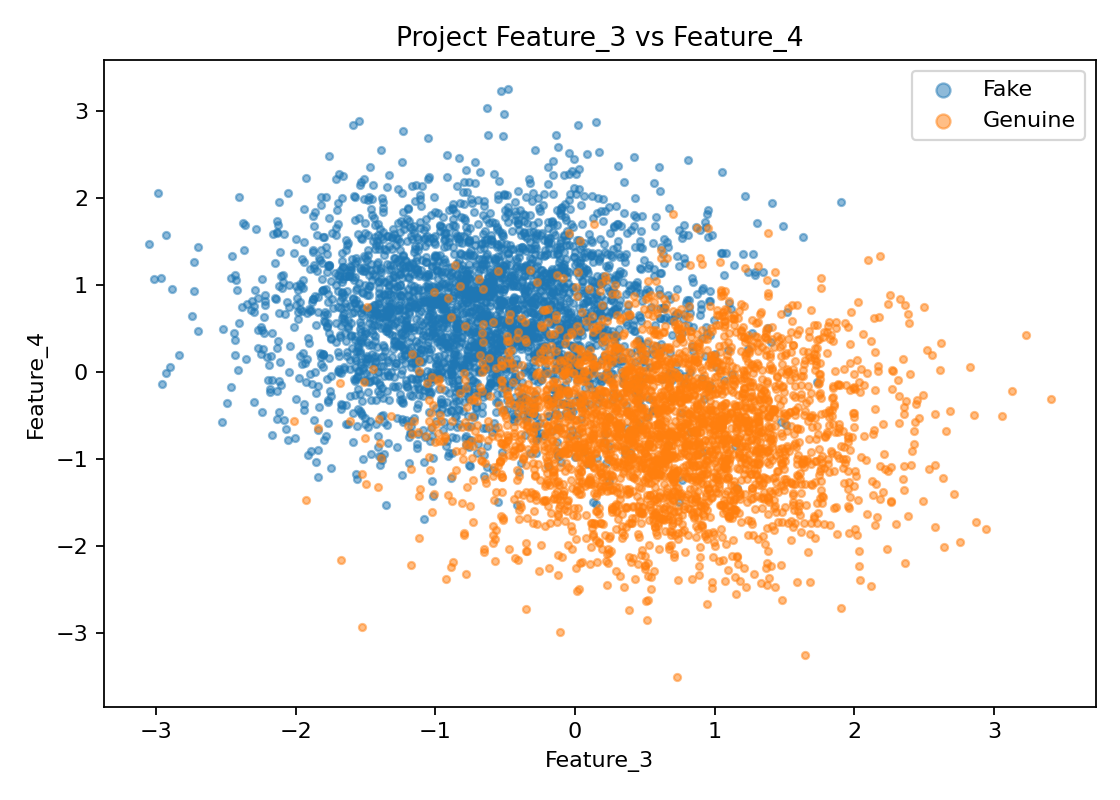
\includegraphics[width=0.6\textwidth]{scatters/features_3_4_scatter.png}
    \caption{Scatter plot of Feature 3 vs Feature 4, illustrating diagonal separation with symmetric class variances.}
    \label{fig:scatter_3_4}
\end{figure}

\subsection*{Theoretical Analysis}

The geometry of Features 3 and 4 represents a "textbook" Gaussian distribution scenario. Because both classes share virtually identical variances across both axes (approximately $\sim 0.54$), their scatter clusters have the exact same geometric "shape"—they are symmetric, roughly spherical clouds of data.

Because their shapes are identical, the classes differentiate themselves entirely through a spatial shift (the translation of their means). The Fake class is shifted to the top-left, and the Genuine class is shifted to the bottom-right, creating the most linearly separable feature pair in the entire dataset.

\subsection*{Motivation and Future Insights}

The "well-behaved" nature of Features 3 and 4 provides a critical counterpoint to the chaotic topology of the other features, offering the following modeling insights:

\begin{enumerate}
    \item \textbf{Suitability for Linear Models:} Because the classes have identical covariance spreads and are separated by a spatial shift, a simple linear decision boundary (such as one generated by Logistic Regression or Linear Discriminant Analysis) would be highly effective if these were the only two features in the dataset. A straight diagonal line cleanly bisecting the space between the centroids would achieve a low error rate.
    \item \textbf{The Tied MVG Trap:} Features 3 and 4 are the only features where the fundamental assumption of the Tied Covariance MVG actually holds true. The Tied MVG assumes that all classes share the exact same covariance matrix. While this assumption is valid for Features 3 and 4, applying it to the entire 6-dimensional dataset forcefully averages the inverted variances of Features 1/2 and destroys the multi-modal clusters of Features 5/6, which explains the catastrophic calibration loss the Tied model suffered in Laboratory 10. 
\end{enumerate}
\newpage

\section{Analysis of Features 5 and 6}

\subsection*{Empirical Results}

To conclude our exploratory analysis, we examine Features 5 and 6. This feature pair is the most topologically complex in the entire dataset and represents a severe departure from standard probabilistic assumptions.

\textbf{Distributions and Overlap:}
Based on the histograms (\texttt{feature\_5\_histogram.png} and \texttt{feature\_6\_histogram.png}), a fundamental asymmetry between the classes emerges. The Fake distribution is unimodal (centered near zero) with wide tails. However, the Genuine distribution is strictly \textbf{bimodal}. It exhibits two distinct peaks with a noticeable "valley" or hollow region in the center where the Fake class peaks. 
Consequently, the classes overlap extensively across almost the entire range of values, but they do so in a highly interleaved, non-linear manner.

\textbf{Statistical Metrics:}
The computed statistics confirm this structural density:
\begin{itemize}
    \item \textbf{Means:} Both classes share nearly identical means centered tightly around zero. For Feature 5, the Fake mean is $0.0280$ and Genuine is $-0.0417$. For Feature 6, the Fake mean is $-0.0058$ and Genuine is $-0.0384$.
    \item \textbf{Variances:} The Genuine class exhibits nearly double the variance of the Fake class on both axes. For Feature 5, Fake variance is $0.6801$ while Genuine is $1.3178$. For Feature 6, Fake variance is $0.7050$ while Genuine is $1.2870$.
\end{itemize}

\begin{figure}[H]
    \centering
    \begin{minipage}{0.48\textwidth}
        \centering
        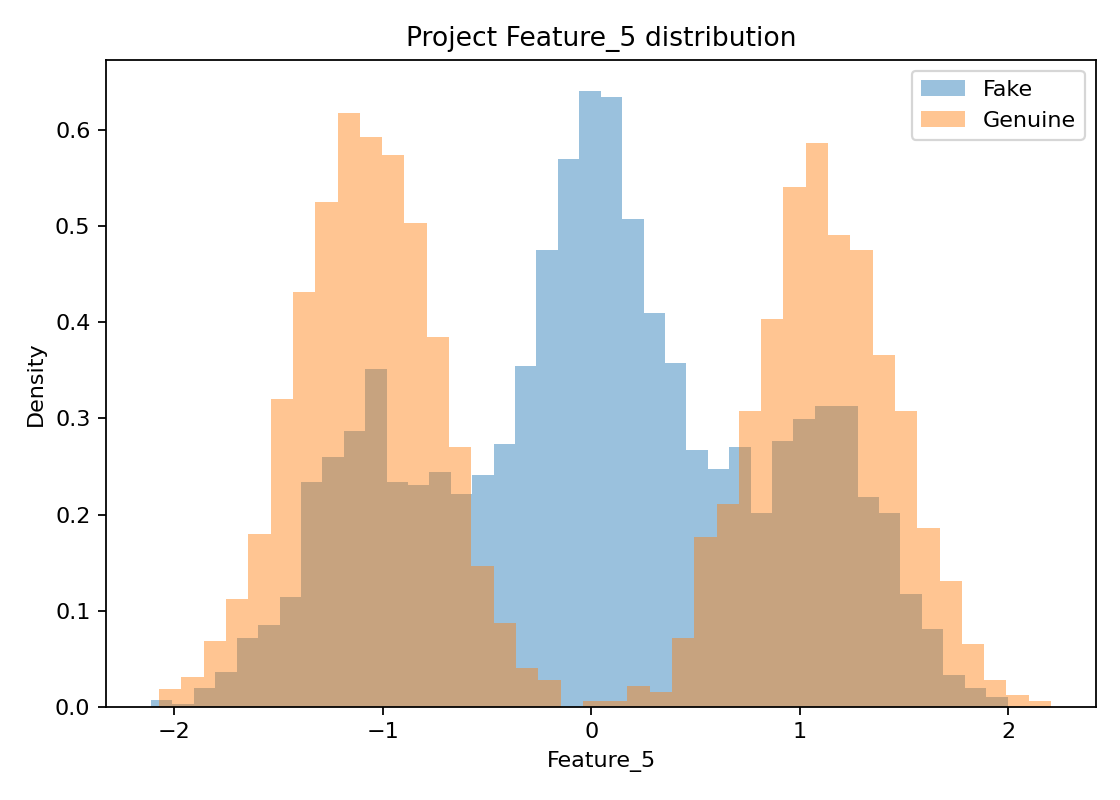
\includegraphics[width=\linewidth]{histograms/feature_5_histogram.png}
        \caption{Histogram of Feature 5, showing Genuine bimodality.}
    \end{minipage}\hfill
    \begin{minipage}{0.48\textwidth}
        \centering
        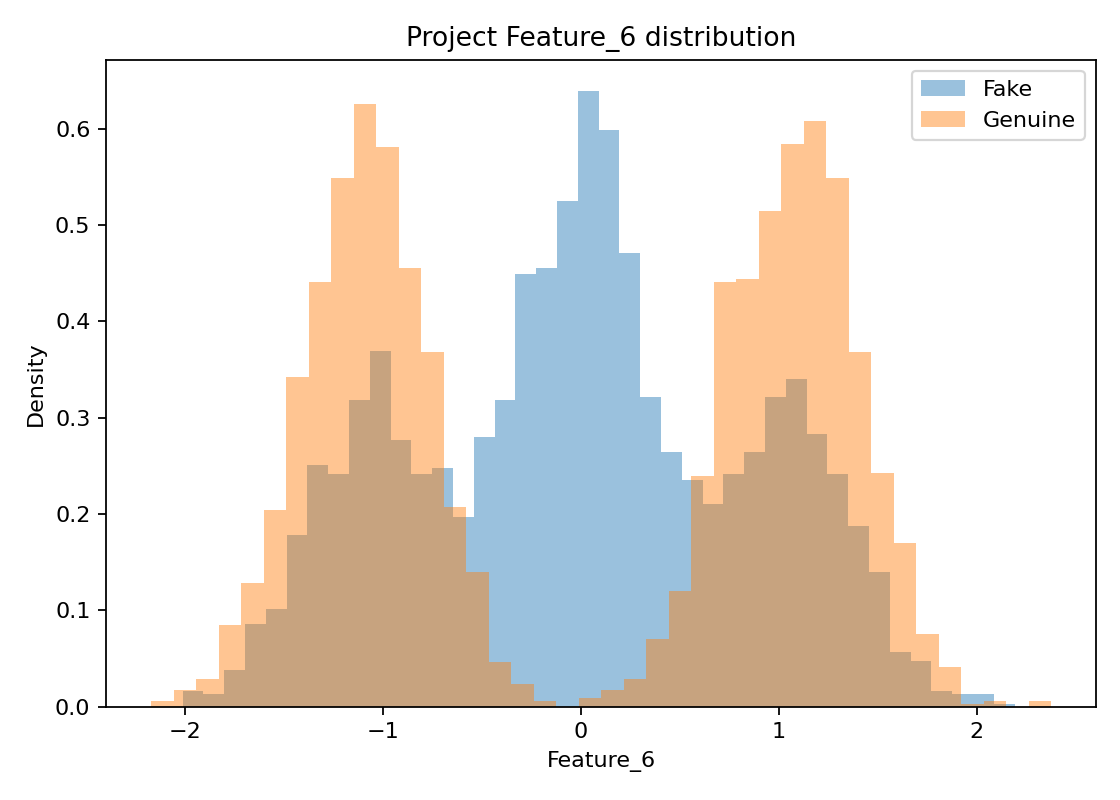
\includegraphics[width=\linewidth]{histograms/feature_6_histogram.png}
        \caption{Histogram of Feature 6, showing Genuine bimodality.}
    \end{minipage}
\end{figure}

\begin{figure}[H]
    \centering
    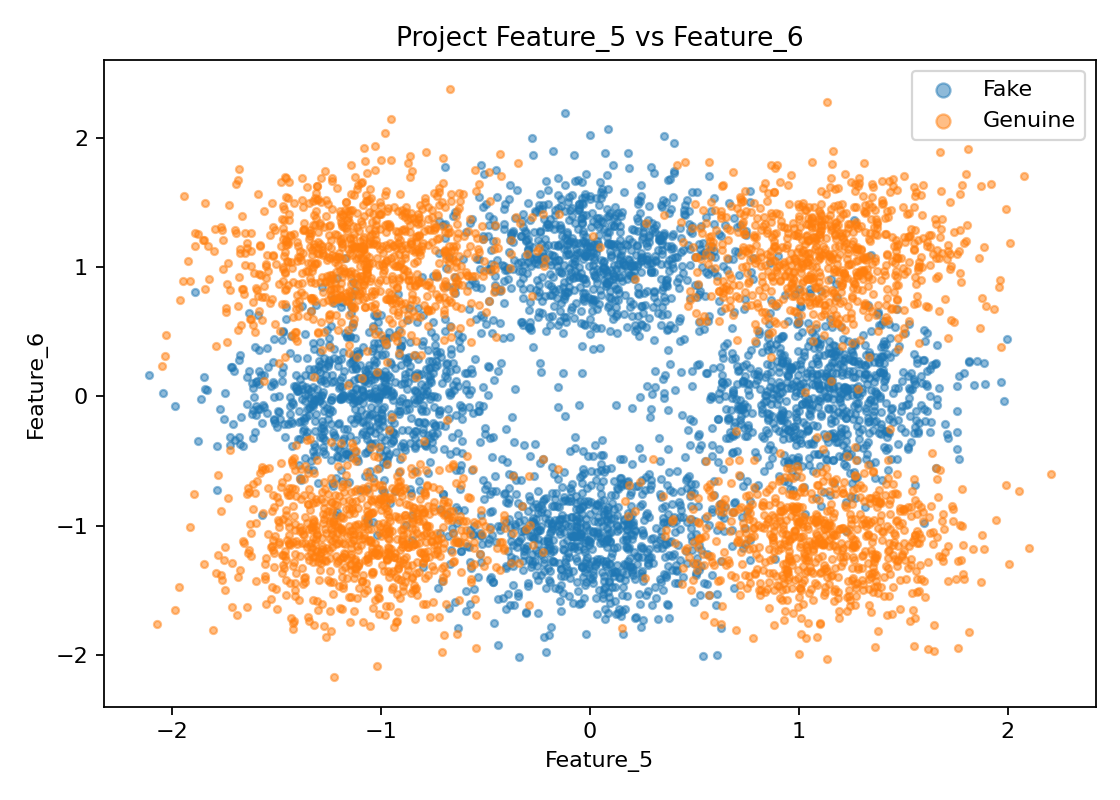
\includegraphics[width=0.6\textwidth]{scatters/features_5_6_scatter.png}
    \caption{Scatter plot of Feature 5 vs Feature 6, illustrating the 4-cluster cross and quadrant topologies.}
    \label{fig:scatter_5_6}
\end{figure}

\subsection*{Theoretical Analysis}

The 2D scatter plot (Figure \ref{fig:scatter_5_6}) resolves the 1D bimodal histograms into explicit, highly structured spatial clusters. Because the Genuine class has distinct peaks at the positive and negative extremes of both axes, it forms a "ring" consisting of exactly \textbf{4 distinct clusters} located in the four diagonal quadrants of the plot (top-left, top-right, bottom-left, bottom-right).

Conversely, the Fake class forms a "cross-like" structure. It also breaks down into roughly \textbf{4 distinct clusters}, but these are located radially along the x and y axes. This creates a geometric grid where the classes interleave perfectly, completely hollowing out the linear separability of the feature space.

\subsection*{Motivation and Future Insights}

The discovery of the 4-cluster topology in Features 5 and 6 is the defining characteristic of this dataset and serves as the mathematical bedrock for our advanced architectural choices in subsequent laboratories:

\begin{enumerate}
    \item \textbf{The Inadequacy of Standard MVG:} A single Multivariate Gaussian distribution (a bell curve) can only model a single center of mass. It cannot physically stretch to cover four isolated quadrants while ignoring the center. Applying a Standard MVG to the Genuine class forces the model to place its mean at $(0,0)$—the exact location of the "valley" where no Genuine data actually exists. This fundamentally compromises the generative log-likelihood estimates.
    \item \textbf{The Necessity of the Gaussian Mixture Model (GMM):} This highly non-Gaussian, multi-cluster topology mathematically necessitates the use of a GMM. By using $M=8$ components (as deployed in our final system), the GMM can assign individual Gaussian spheres to each of the distinct corner clusters, perfectly mapping the true underlying density contours.
    \item \textbf{The Power of the RBF Kernel:} For discriminative models, linear boundaries cannot navigate this grid-like overlap. The Support Vector Machine requires the non-linear projection of the Radial Basis Function (RBF) kernel to draw localized, circular boundaries capable of "wrapping around" the isolated Genuine clusters. This geometrically proves why the GMM and RBF SVM fusion in Laboratory 10 achieved the optimal Minimum DCF.
\end{enumerate}

\end{document}
